
\section{Background}
\label{sec:background}



\subsection{M-learning and the Teaching of Programming}

Mobile devices can be used for fun, entertainment, communication and learning, among many other possibilities. They provide a more personal experience, besides being cheaper than desktops computers \cite{ juniortowards}. Moreover, they can be adopted as a way to carry the classrooms lessons for learners' houses \cite{20123315330601}. 

The number of applications for education has growing significantly. However, most of such applications support only informal learning \cite{marcolino_edu2015}. Besides that, there are many issues to overcome and to address for allowing the use of mobile devices' potential in the education in several areas, such as in teaching of programming \cite{marcolino_edu2015, tedesco2012}.

Despite the programming domain has growing and that many countries are changing their primary and secondary curricula for including programming disciplines, such domain still faces several problems \cite{Duncan:2014:YLC:2670757.2670774}. Based on the analysis of applications for the teaching of programming, we noticed the need of improvement of the support for teachers in classrooms, the providing of more accurate feedback for the learners and the creation of more engaging environments \cite{marcolino_edu2015, tedesco2012, Duncan:2014:YLC:2670757.2670774}. 

Based on these issues and on the need of evolving the learning applications, exploring their features systematically, an SPL to create mobile learning applications for the teaching of programming foundations has been proposed \cite{marcolinoarcht2017}. 

\subsection{The M-learning SPL}

The proposed SPL follows the SPLE (Software Product Line Engineering) framework \cite{pohl2005}. Composed of nine-sub process, the SPLE describes the main activities and artifacts of each subprocess, easing the conduction of the SPL life-cycles, namely: domain engineering and application engineering. Marcolino e Barbosa \cite{marcolinoarcht2017} specified each phase in the creation of an M-learning SPL, its conceptual architecture and proposed improvements in the first three SPLE sub-process. Figure \ref{fig:schema} presents the SPL conceptual architecture.

%At the top of Figure \ref{fig:schema} is the SPLE framework and its layers. The interaction between domain engineering life-cycle and application mechanism (green arrow) supports the creation of applications. Application mechanism interacts with the application engineering life-cycle for the creation of m-learning applications for the teaching of programming (blue arrow), which reduces the amount of technical support.

%The blue arrow (Figure \ref{fig:schema}) specifies 

In Figure \ref{fig:schema}, the m-learning applications architecture presents the mobile client application, that provides a macro view of Presentation Layer, Service Layer, Business Layer (Educational and Programming), Data Layer (persistence) and Cross-Cutting/Orthogonal Services Layer and their interactions with external elements, External Infrastructure and External Sources.

\begin{figure*}[!ht]
    \centering
    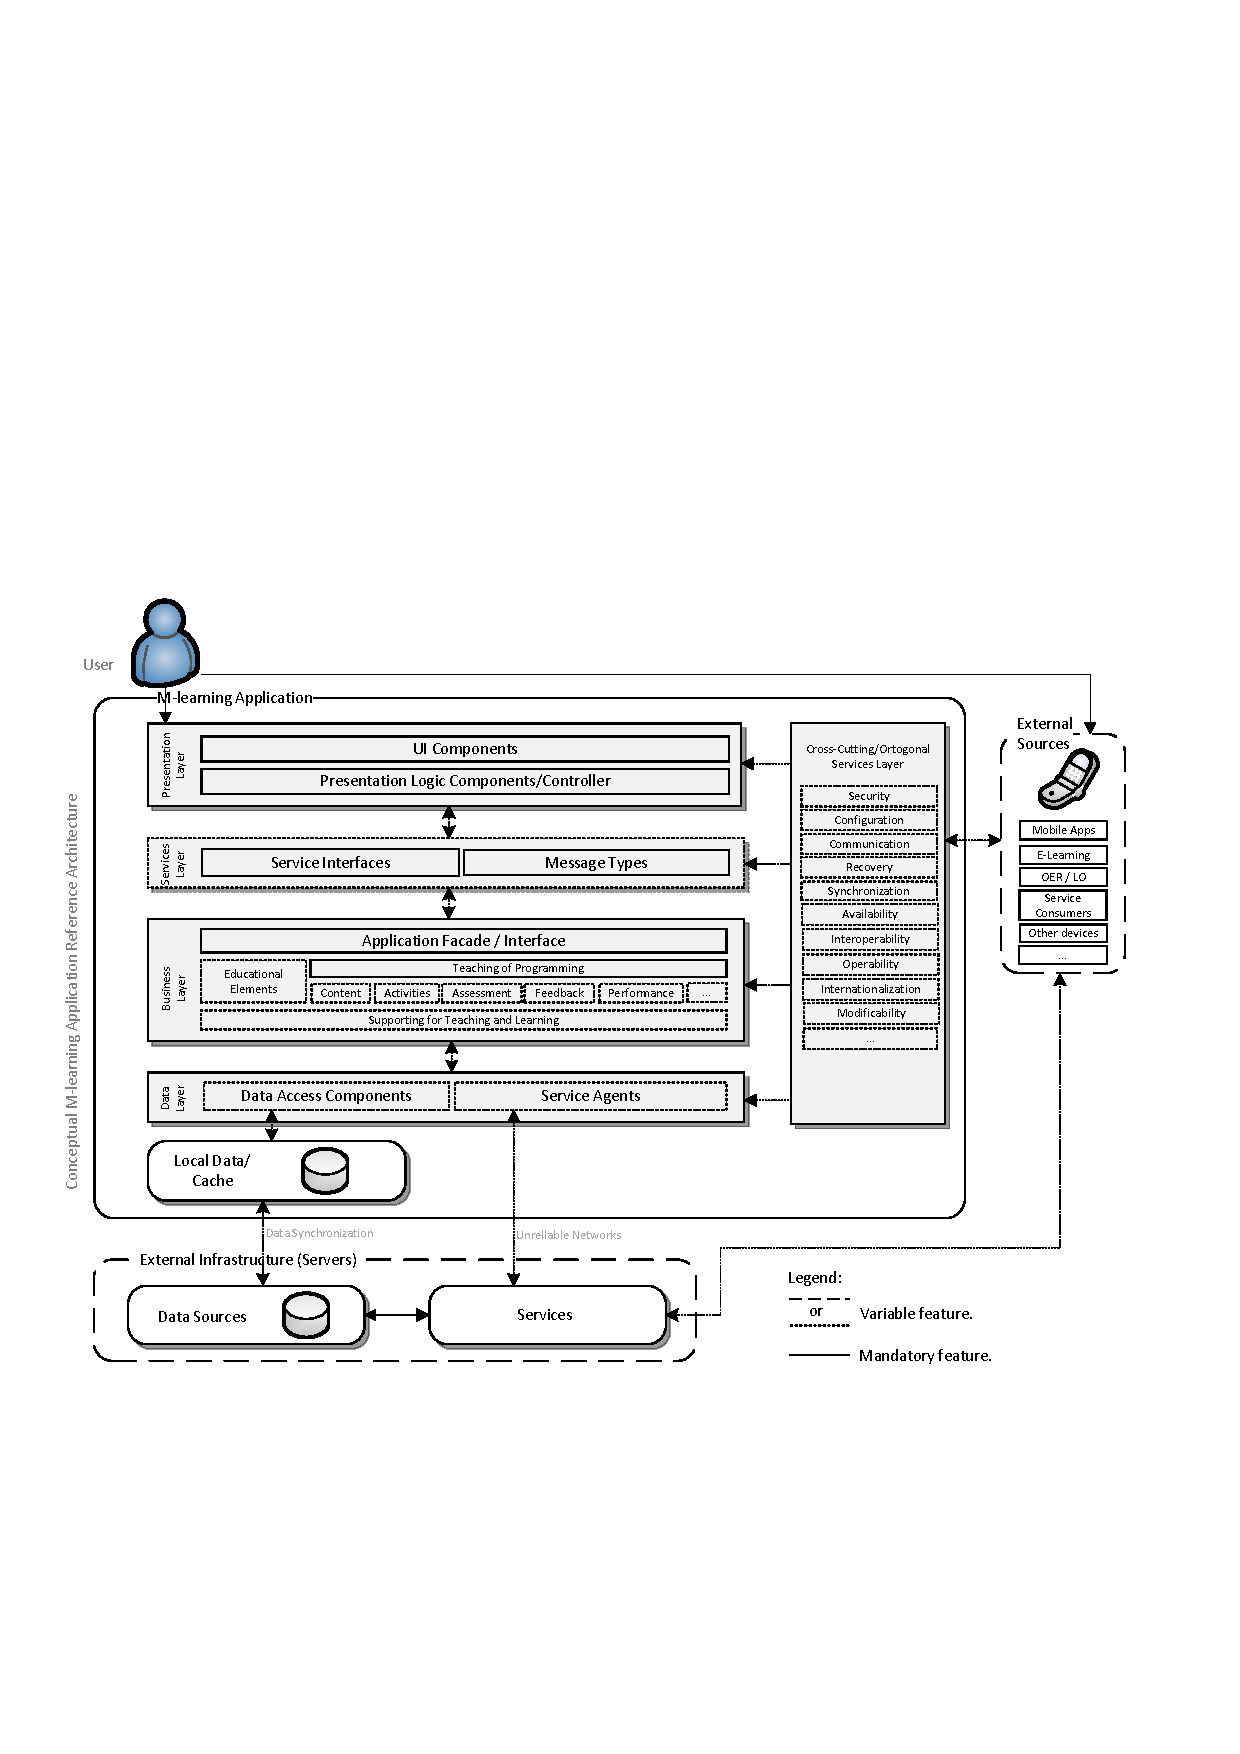
\includegraphics[scale=0.75]{conceptual_old.pdf}
    \caption{M-learning SPL Conceptual Architecture Excerpt \cite{marcolinoarcht2017}.}
    \label{fig:schema}
\end{figure*}

%The three green subprocess (Figure \ref{fig:schema}): Project Management, Domain Requirements Engineering and Domain Design were conducted. This last subprocess was concluded until the logical view through the feature model and the conceptual architecture model. 

The Domain design differs from design of single systems mainly because it incorporates configurations mechanisms into the SPL reference architecture to support the variability of product line, this mechanisms are presented in \cite{marcolinoarcht2017} and are considered in the final SPL solution. Furthermore, it allows the development of an adaptable architecture for future inclusion of new features and designates the reusable parts with no loose of rules for the development of specific applications based on the SPL reference architecture.

However, the evaluation conducted with 31 main stakeholders involved in the process did not consider the industry practitioners. Such stakeholders were from academic area, having know--how in software engineering, programming, m-learning and mobile development. Therefore, a re-analysis in practitioners perspectives is needed before the SPL architecture representation in the development and process views, in which both will be supported by the SMarty approach. The aim is evolve the already evaluated architecture to attenuate possible future problems in development phase.


\subsection{The SMarty Approach}


The SPLE framework designates the adoption of the orthogonal variability model \cite{pohl2005}. However, this model adopt a specific graphic notation, requiring the understanding of the notation to be applied. Additionally, the creation of such models needs specific modeling tools for the conception of them. To minimize the inclusion of a new notation for developers and to easy the process of understanding for industry practitioners, the SMarty approach was adopted in the conception of the SPL models \cite{deOliveira2013, marcolino2013}.


SMarty supports the representation and management of variability in UML models. It supports use case, sequence, class, activity and component UML models through an UML 2 profile, named \textit{SMartyProfile}. UML profile allows an easier integration of their notation in any modeling tool that enables UML profiles import. SMarty also provides the \textit{SMartyProcess}, a set of guidelines that guide users in its application, providing also the support for the detection of (new) features in UML models.

The \textit{SMartyProfile} comprises the following stereotypes: $\ll$variability$\gg$, $\ll$mandatory$\gg$, $\ll$optional$\gg$, $\ll$alternative\_OR$\gg$, $\ll$alternative\_XO$\gg$; $\ll$mutex$\gg$ and $\ll$requires$\gg$. It also has a set of attributes for presenting extra and fundamental information such as the rastreability among the variabilities, the maximum and minimum number of variants, all of them included in an UML comment element.


Finally, other reason for the selection of SMarty was the good results of a set of experimental evaluations, where it was compared the process of identification of variability with UML-based Software Engineering Method (PLUS) and Ziadi et al. approach \cite{marcolino2013, MarcolinoJG14}. Even with a better representation of PLUS method in Class models, mainly by the set of reduced stereotypes, SMarty showed to be the best choice because of its set of guidelines. Moreover, as the approach allows the management of their stereotypes in a profile, the addition of new syntactic elements is facilitated \cite{deOliveira2013}, enabling the constant evolution of SPL core assets.
